% Sections/3_further_investigation.tex
\section{Further Investigation}

To answer the overarching research question, this chapter focuses on two practical investigations. 

\begin{enumerate}
    \item \textbf{Annotation Workflow Audit} \\
    \textbf{HMW:} How might we identify the mechanical bottlenecks in current dataset creation tools that prevent the scalable, metadata-rich annotation of image detection datasets? \\
    \textbf{Objective:} To investigate how to create vape data, then audit industry-standard computer vision annotation platforms from a functional and User Experience (UX) perspective.

    \item \textbf{Frontline Operations Interviews} \\
    \textbf{HMW:} How might we understand the daily routines and constraints of municipal cleaners to ensure UAV detections translate into intuitive and actionable cleanup interventions? \\
    \textbf{Objective:} To evaluate the current municipal landscape from a Human-Centered Design (HCD) perspective. Through semi-structured interviews with five frontline cleaning staff and operational managers, this investigation maps standard litter operating procedures to determine manual bottlenecks and inefficiencies in cleaning plans.
\end{enumerate}

\subsection{Annotation Workflow Audit}

To evaluate their suitability for UAV-based micro-litter preprocessing, a functional audit was conducted across five leading annotation platforms: Roboflow, Ultralytics Hub, CVAT, Label Studio, and V7 Darwin \cite{roboflow_docs,ultralytics_platform_docs,cvat_docs,labelstudio_docs,v7darwin_product}. This investigation analysed the comparative advantages and operational bottlenecks of each tool during dataset preparation. It is acknowledged that this heuristic evaluation represents a single-user perspective; however, this focused approach allowed for a deeply granular analysis of the mechanical and UX boundaries governing each platform. A comprehensive evaluation matrix detailing these platform specifics is provided in Table~\ref{tab:appendix_annotation_tool_benchmark}, the averaged results of which were synthesised into a dataset construction user journey map.

\begin{figure}[H]
    \centering
    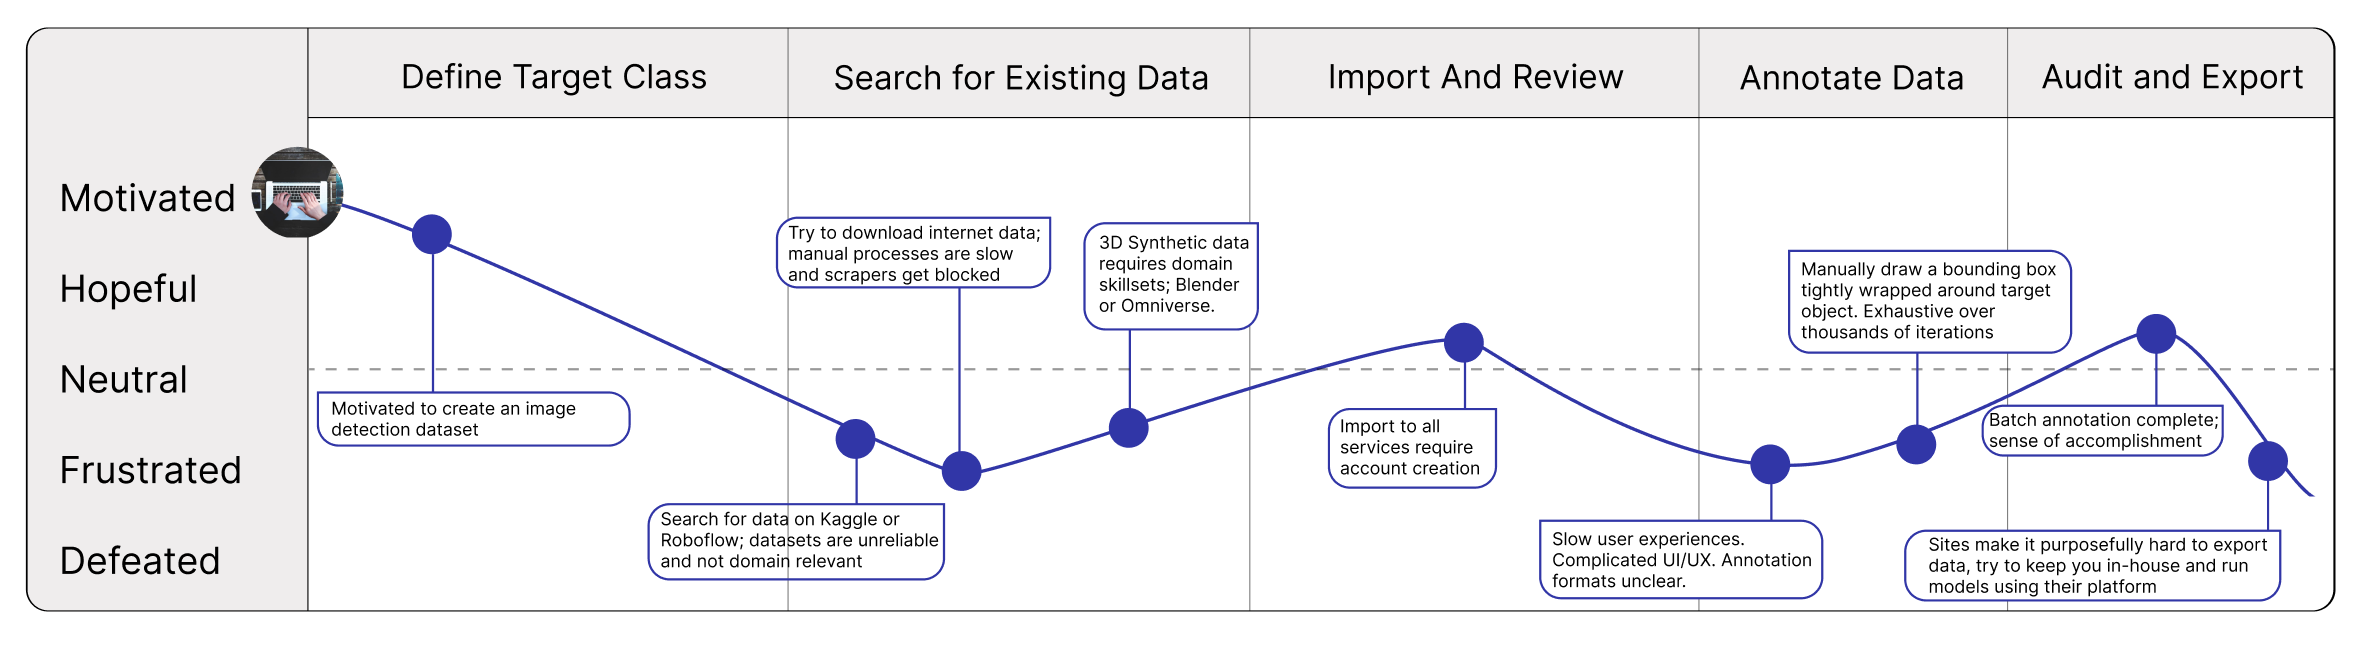
\includegraphics[width=0.8\linewidth]{annotate_userflow.png}
    \caption{Annotation Workflow, User Journey Map}
    \label{fig:annotation_userflow}
\end{figure}

Mapping this journey exposed severe effort/friction "lows," revealing that current platforms are designed strictly as \textit{annotation} tools, not dataset \textit{creation} engines.

\textbf{The Sourcing \& Discovery Bottleneck:} 
Current tools operate on the assumption that a raw dataset already exists. However, an initial repository search confirmed the complete absence of an open-source, UAV-oriented vape-litter dataset. Consequently, the user journey begins with a severe friction point: data sourcing. Platforms offer virtually no native scraping or raw data ingestion pipelines. While repositories like Roboflow Universe provide community datasets for common objects, they offer no support for niche, emerging hazards. Furthermore, synthetic data generation is entirely fragmented from the annotation ecosystem, forcing users into disconnected external workflows (e.g. Blender, NVIDIA Omniverse, or custom Python scripts) before annotation can even begin. 

\textbf{Walled Gardens and Model Abstraction:} 
Once data is finally sourced and imported, many commercial platforms function as walled gardens. They typically encourage platform lock-in through mandatory account creation, cloud hosting or usage limits, while local export formats can feel secondary to the hosted workflow. Moreover, while these platforms have recently integrated semi-automated annotation tools, these capabilities may sit behind commercial quotas or paid tiers. This platform abstraction can also obscure which underlying model is being used, reducing scientific transparency when the user needs a reproducible annotation pipeline. 

\textbf{UX Friction in Batch Processing:} 
The audit highlighted critical usability bottlenecks during the annotation phase. For micro-objects like disposable vapes, high-volume dataset creation requires low-friction, rapid interaction. Instead, many modern interfaces resemble general-purpose image editors with a feature-rich interface. The cumulative time lost to minor GUI actions: manually switching tools, zooming into different parts of images, dragging a cursor and clicking on different buttons, and inefficiently navigating between different images for audit purposes is highly inefficient. A minimal, hotkey-driven workflow optimized for rapid batch processing would be more ideal for batch annotating.

\textbf{Manual Metadata Tagging:} 
Finally, tools rarely support metadata tagging for each image. Metadata, contextual image variables (e.g. weather, altitude, lighting), are typically user inputted as rigid image tags or not included as an input option entirely. While metadata are niche in image detection workflows, the inclusion of them, especially in the context of UAV models, would greatly explain failure modes, improving iteration attempts of deep-learning models.

\subsection{UK Cleaners Investigation}

Primary qualitative research was conducted with five UK litter cleaners: three community volunteers the Canal \& River Trust and Keep Britain Tidy, and two contracted operatives from Veolia UK to provide critical frontline insights. It is acknowledged that these samples serve as contextual, exploratory, qualitative evidence rather than a formal cleaner study. To synthesize these findings, two representative personas were developed: the community volunteer (P1) and the paid street operative (P2). 

\begin{figure}[H]
    \centering
    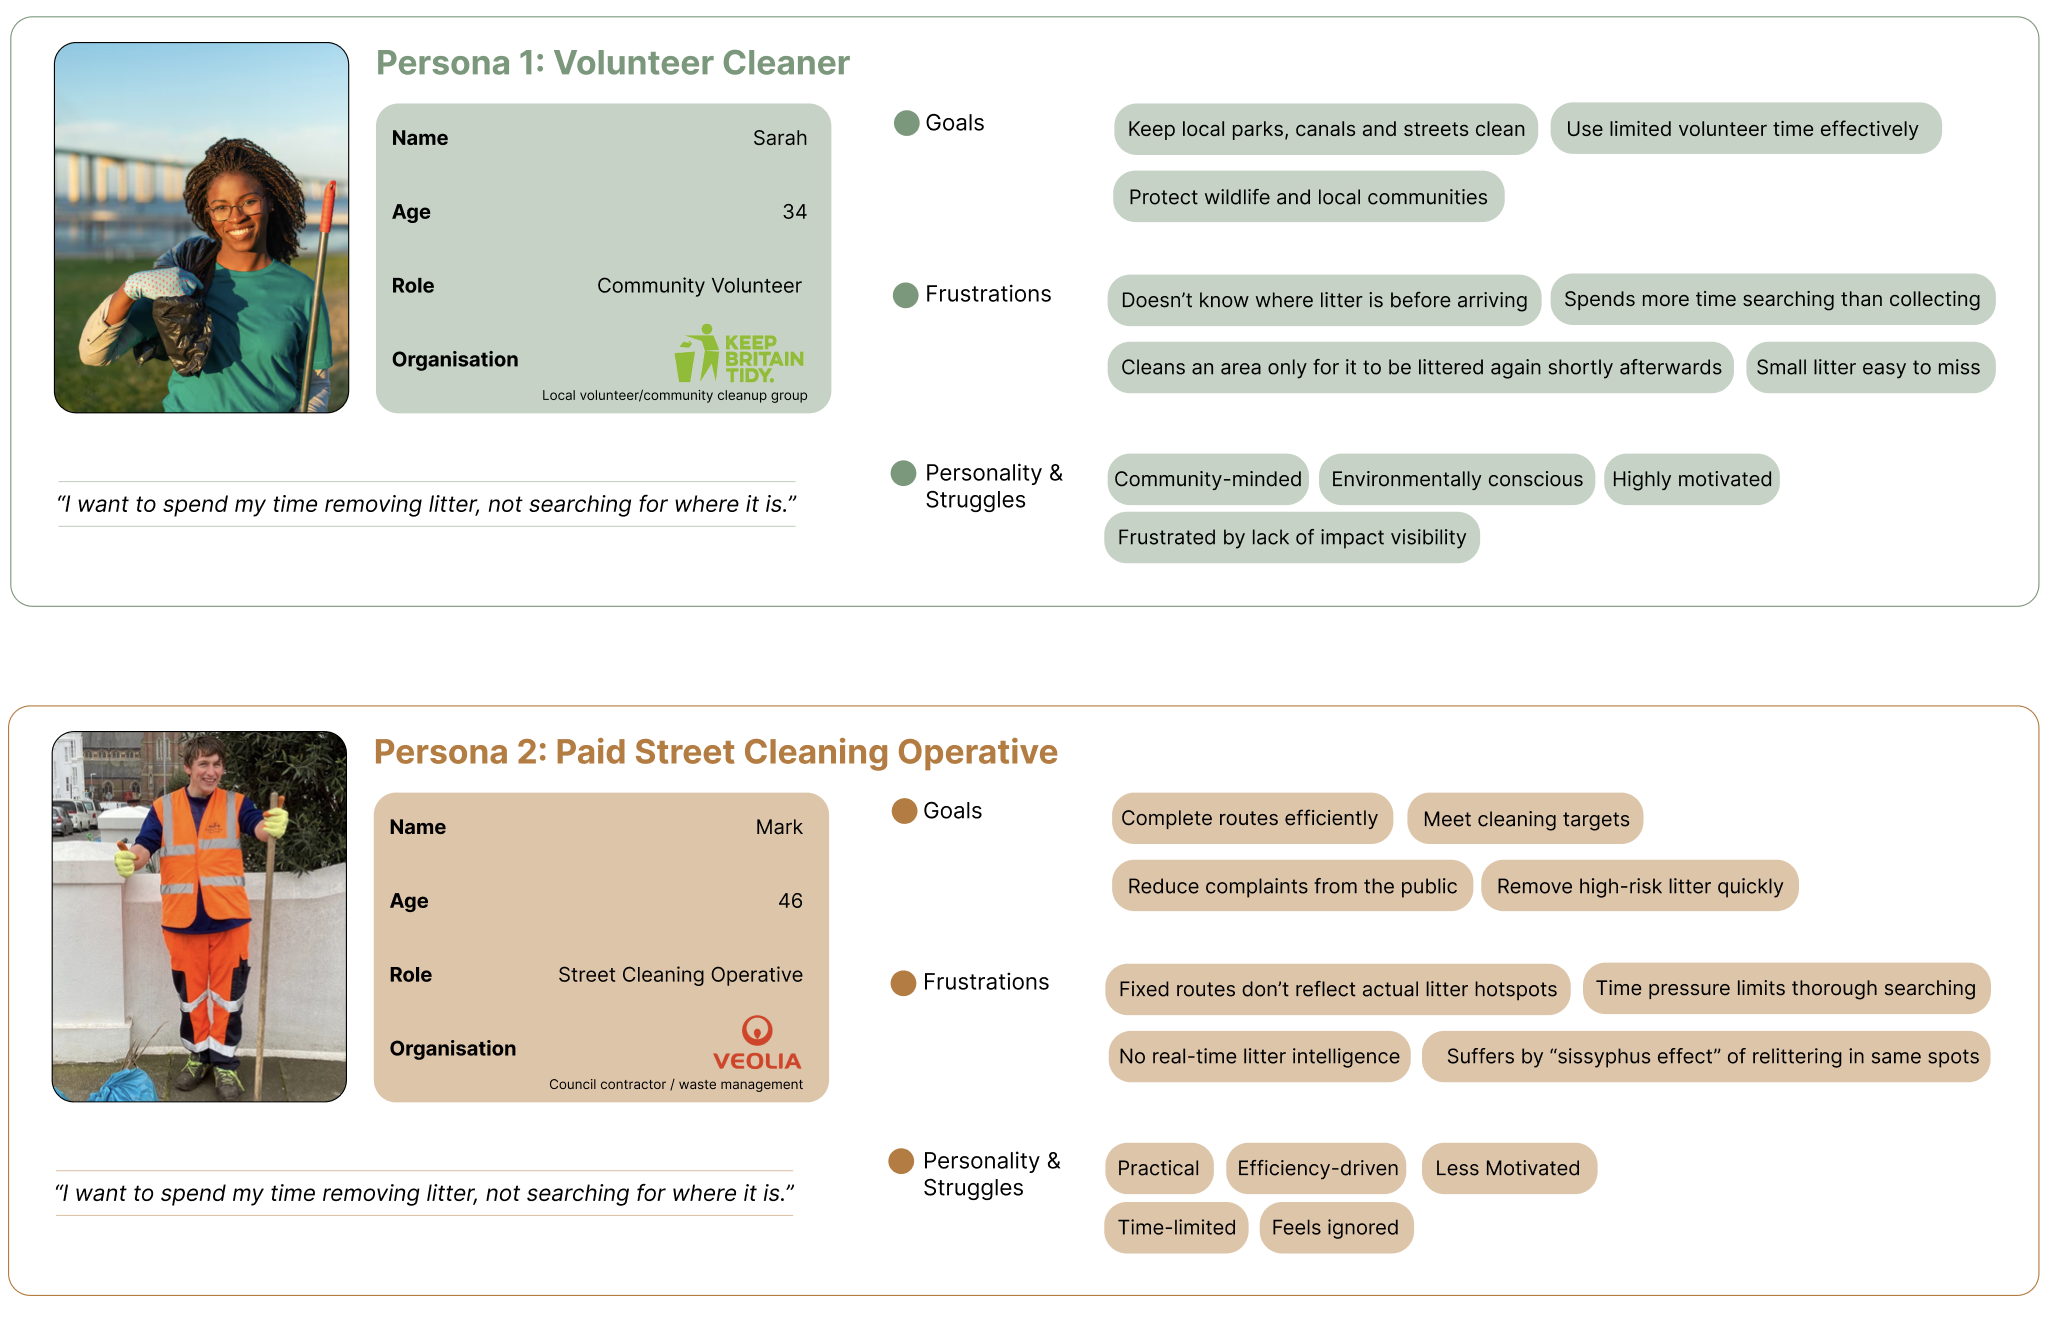
\includegraphics[width=0.8\linewidth]{Screenshot 2026-06-02 at 06.57.59.png}
    \caption{User Personas: Community Volunteer (P1) and Contracted Cleaner (P2)}
    \label{fig:cleaner_personas}
\end{figure}

\begin{figure}[H]
    \centering
    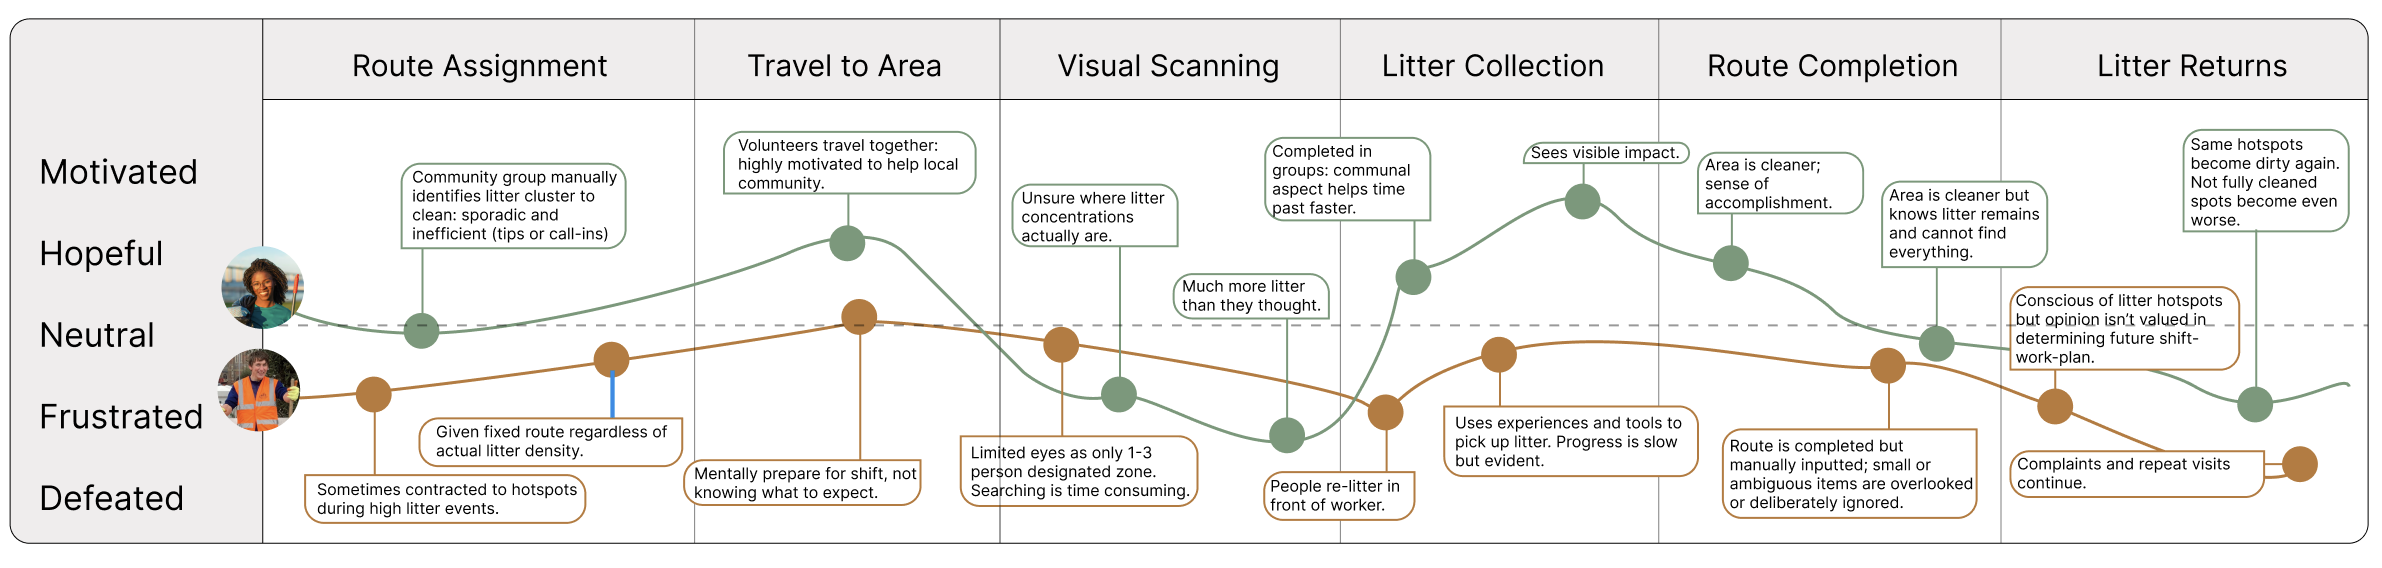
\includegraphics[width=0.8\linewidth]{Figures/User_Journey.png}
    \caption{P1 and P2 User Journey Map}
    \label{fig:cleaner_user_journey}
\end{figure}

An analysis of their current-state cleaning journey reveals systemic failures in how litter is managed in UK urban environments and untapped technological opportunities.

\vspace{1em}
\noindent\textbf{The Visibility Bottleneck and the ``Sisyphus Effect''}

The journey map indicates that the primary bottleneck in litter management is workflow inefficiencies. Before a shift even begins, work plans and routes are often manually planned or rigidly fixed using static maps, with no dynamic intelligence on where litter actually is on that given day. P2 may often know where hotspots are, but are forced to abide to shift-work-plans. Once on the ground, cleaners must rely on slow, unguided visual scanning, searching step-by-step along these fixed routes, wasting significant time. Further, cleaners suffer from a "Sisyphus effect": as cleaners only verbally verify cleaned hot-spots, areas are superficially cleaned only to be immediately re-littered, causing operative frustration.

\vspace{1em}
\noindent\textbf{The Micro-WEEE Systemic Failure}

In-person cleans revealed that while severe hazards like syringes or knives trigger specific safety protocols, disposable vapes are not consistently treated as hazardous. Volunteer cleaners were largely unaware that e-waste such as vapes or lighters cannot be disposed of in standard public bins or general recycling. Legally, they must be deposited in dedicated WEEE bins or returned to retailers. While a crossed-out wheelie bin logo indicates this requirement, it is imprinted so microscopically on the base of the device that cleaners and consumers miss it.

\begin{figure}[H]
    \centering
    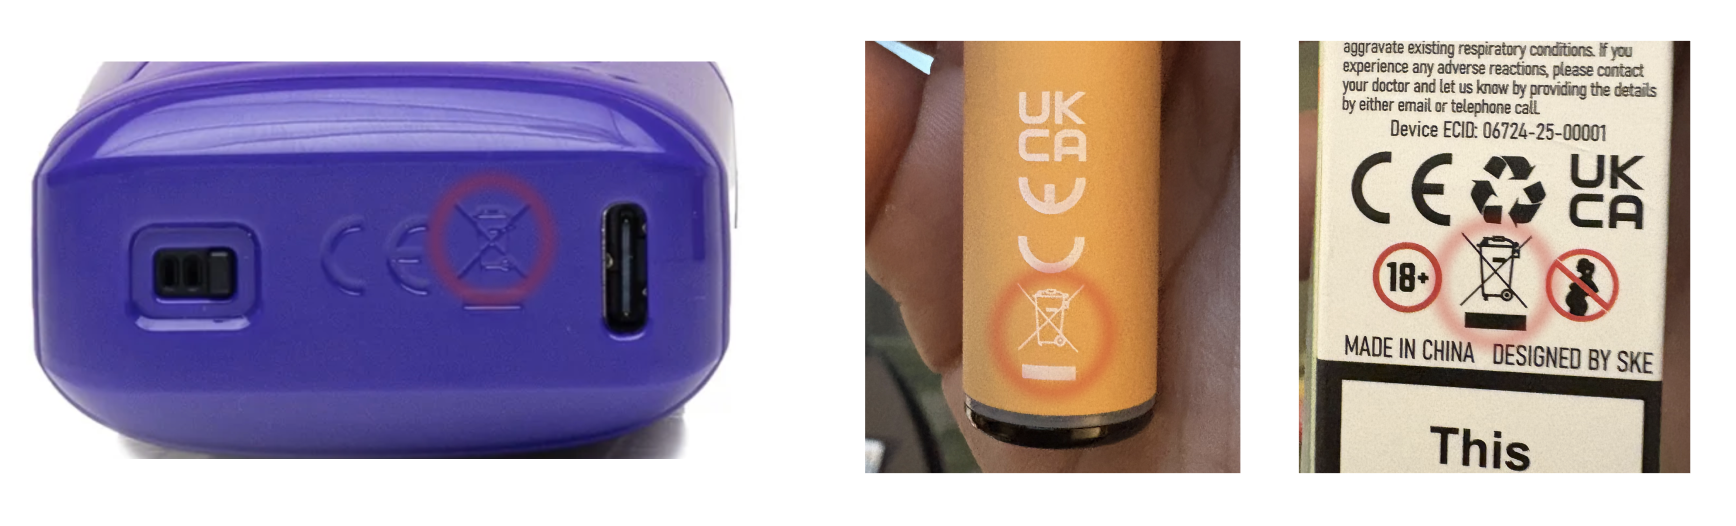
\includegraphics[width=0.5\linewidth]{Vape Disposal Labels.png}
    \caption{Vape Disposal Labels}
    \label{fig:vape_disposal_labels}
\end{figure}

Further, dedicated electronics recycling bins are rarely visible in urban environments, if at all known to any cleaner. Informal investigations of local retailers, ranging from major supermarkets like Tesco to dedicated vape shops, revealed that staff were frequently unaware of their own mandatory take-back schemes, reporting that they had never experienced a customer vape return. So even an attempted proper retail disposal may be futile.  This systemic issue highlights that any cleaning solution must distinguish vapes as a hazardous litter class with distinct clean-up steps to normal litter.

\vspace{1em}
\noindent\textbf{The Smartphone Opportunity and Evidence-Backed Tasking}

Importantly, both volunteers and contracted cleaners carry and use smartphones during their shifts. Some volunteer groups, such as the Canal and River Trust, use smartphones to take photos of litter and report it in WhatsApp groups, while others use phones for non-work-related tasks. However, none of the participants described using a dedicated tool to streamline the cleaning process itself. This makes software-supported reporting and tasking plausible, while still requiring prototype validation.

\subsection{Investigation Synthesis}

Drawing back to the research question:
\vspace{0.5em}
\noindent\textbf{How might we overcome the structural barriers to identifying and operationalizing disposable vapes as hazardous micro-e-waste in UAV-oriented imagery for UK urban environments?}

We found that commercial annotation platforms function primarily as proprietary walled gardens designed to host and monetize existing data, rather than end-to-end dataset creation engines. By treating annotation as a general-purpose commercial editing task, these services completely neglect initial data sourcing, restrict rapid batch-processing through poor UX, and omit the environmental metadata crucial for UAV failure-mode analysis. Consequently, to build a novel micro-WEEE dataset, these fragmented tools must be bypassed in favour of a dedicated, locally hosted, and hotkey-driven dataset construction workflow.

Further, the current municipal cleanup workflow is severely bottlenecked by rigid, blind-sweep routing and a systemic failure to recognize or properly dispose of micro-WEEE. However, the ubiquitous presence of smartphones among frontline cleaners presents an untapped platform for evidence-backed tasking. To bridge the gap between UAV detection and physical removal, a mobile-first UI must translate static spatial heatmaps into dynamic interventions. This system must move beyond merely showing \textit{where} litter is; it must prioritize dynamic routing to eliminate the ``Sisyphus effect,'' explicitly preserve the vape's identity to instruct operatives on \textit{what} the hazard is, and provide a verifiable pathway for proper e-waste disposal.

Therefore, the project scope has matured from a standalone computer vision task into an interdisciplinary systems-thinking project, comprising three integrated workstreams:

\begin{itemize}
    \item \textbf{Dataset Construction Engine (DCE):} The data infrastructure required to make fragmented vape and litter imagery curated, metadata-rich, auditable, and model-ready.
    \item \textbf{UAVape Dataset and Detector:} The application of that infrastructure to build a micro-WEEE dataset and benchmark a YOLO-family detector.
    \item \textbf{Cleanup Planner Prototype:} The UI prototyping required to translate vape detections into an evidence-backed tasking interface for municipal cleaners.
\end{itemize}
